\chapter{Representation theory}
A complex vector space $V$ can be thought of as an Abelian group, where the group product is denoted by ``$+$'' and called  ``sum'', and the neutral element is denoted as $\vo$, and in which an additional operation, called ``scalar multiplication'' by a complex number $\mu \in \C$ has been defined, such that the following conditions are satisfied:
\begin{enumerate}
    \item $\mu(\vv_1 + \vv_2) = \mu\vv_1 + \mu\vv_2$;
    \item $(\mu_1 + \mu_2)\vv = \mu_1\vv + \mu_2\vv$;
    \item $\mu_1(\mu_2\vv) = (\mu_1\mu_2)\vv$;
    \item $1\vv = \vv$;
    \item $0\vv = \vo$.
\end{enumerate}
One could have also replaced complex numbers with real numbers to define a ``real vector space''. However, the focus on complex vector spaces is justified by their relevance in quantum mechanics.
\begin{defn}[linear independence]
    Given a linear combination of $k$ vectors $\vv_1,\dots,\vv_k \in V$ of the form $\sum_{i=1}^n\mu_i\vv_i$, the set of vectors $\{\vv_1,\dots,\vv_k\}$ is said to be linear independent if $\sum_{i=1}^n\mu_i\vv_i = 0$ only when all coefficients $\mu_i$ are simultaneously zero. 
\end{defn}
The dimension of a vector space $V$, denoted as $\dim{V}$, is the maximum number of vectors of $V$ that are linearly independent; if $\dim{V} = n$ then the set $\{\ve_1,\dots,\ve_n\}$ of linearly independent vectors of $V$ is called a ``basis'' of the vector space. Given a basis, any vector $\vv \in V$ can be written in a form $\vv = \sum_{i=1}^nv_i\ve_i$, where $v_i$ are the ``components'' of the vector and are fixed uniquely. 
\begin{defn}[linear map]
    Given two vector spaces $V_1$ and $V_2$, a map $L : V_1 \to V_2$ is said to be a linear map if it satisfies 
    \begin{equation}
        L(\mu_1\vv_1 + \mu_2\vv_2) = \mu_1L(\vv_1) + \mu_2L(\vv_2),\quad \forall \mu_1,\mu_2 \in \C,\,\forall \vv_1,\vv_2 \in V.
    \end{equation}
\end{defn}
If a linear map is a bijection, then it is called an isomorphism, and the vector spaces $V_1$ and $V_2$ are said to be isomorphic to each other, $V_1 \simeq V_2$. An isomorphism form $V$ to itself is called an automorphism. The set of automorphism of $V$ is denoted ad $Aut(V)$; it is a group, with composition of mapping $L \circ L'$ as the group product. The neutral element in $Aut(V)$ is the identity automorphism; the existence of the inverse of every automorphism is guaranteed, since automorphism, being isomorphism, are bijections. 
\begin{defn}[image of a linear map]
\label{defn: kernel of a linear map}
    Given a linear map $L : V_1 \to V_2$, the image of $L$ is 
    \begin{equation}
        \im{L} = \{L(\vv_1) : \vv_1 \in V_1\} \subseteq V_2.
    \end{equation}
\end{defn}
\begin{defn}[kernel of a linear map]
\label{defn: image of a linear map}
    Given a linear map $L : V_1 \to V_2$, the kernel of $L$ is 
    \begin{equation}
        \ker{L} = \{\vv_1 \in V_1 : L(\vv_1) = \vo_2\} \subseteq V_1.
    \end{equation}
\end{defn}
It is not difficult to see that the image and the kernel of a linear map are vectors spaces. The following theorems are useful.
\begin{teo}
    Given a linear map $L : V_1 \to V_2$, the dimension $\dim{V_1}$ satisfies $\dim{V_1} = \dim{(\ker{L})} + \dim{(\im{L})}$.
\end{teo}
\begin{teo}
    A linear map $L : V_1 \to V_2$ is an automorphism if and only if $\ker{L} = \{\vo\}$.
\end{teo}
Every linear map is defined uniquely by its action on the basis vectors 
\begin{equation}
    L(\vv) = L\bigg(\sum_{i=1}^nv_i\ve_i\bigg) = \sum_{i=1}^nv_iL(\ve_i),
\end{equation}
one can then expand the vectors $L(\ve_i)$ in the basis $\{\ve_i,\dots,\ve_n\}$, denoting the components by $L_{ij}$, to write $L(\ve_i) = \sum_{j=1}^nL_{ji}\ve_j$, thus
\begin{equation}
    L(\vv) = \sum_{i=1}^n\sum_{j=1}^nv_iL_{ji}\ve_j = \sum_{j=1}^n\bigg(\sum_{i=1}^nL_{ji}v_i\bigg)\ve_j,
\end{equation}
and so the image vector $L(\vv)$ has components $L(\vv)_j = \sum_{i=1}^nL_{ji}v_i$. In the case where $\dim{V_1} = \dim{V_2} = n$, then in the matrix notation one have
\begin{equation}
    \begin{pmatrix}
        L(\vv)_1 \\
        \vdots \\
        L(\vv)_n
    \end{pmatrix}
    =
    \begin{pmatrix}
        L_{11} & \cdots & L_{1n} \\
        \vdots & \ddots & \vdots \\
        L_{n1} & \cdots & L_{nn}
    \end{pmatrix}
    \begin{pmatrix}
        v_1 \\
        \vdots \\
        v_n
    \end{pmatrix}.
\end{equation}
From this one can deduce that the group of automorphism of $V$ is isomorphic to the group of invertible $n \times n$ complex matrix.
\begin{equation}
    Aut(V) = \{L : V \to V : L\mathrm{\,is\,an\,automorphism}\} \simeq GL(n,\C),
\end{equation}
where the group multiplication laws are the composition of maps and matrix multiplication. 

Now that the tools are there, it is possible to give a definition of a representation of a group. The idea is to define the action of a group $G$ on a vector space $V$. If $V$ were just a set, one would associate with every group element $g \in G$ a permutation $L_g \in \Perm{V}$. However, the vector space structure of $V$ has to be preserved. So the action is defined just as before, but replace the group $\Perm{V}$ of permutations of $V$ by the group $Aut(V)$ of automorphism of $V$. 
\begin{defn}[linear representation]
    A linear representation of a group $G$ in a vector space $V$ is a homomorphism $D : G \to Aut(V)$, $g\mapsto D(g)$.
\end{defn}
The dimension of the representation coincides with the dimension of the vector space $V$; also, one can observe that
\begin{enumerate}
    \item since the representation $D$ is a homomorphism,  for any $g_1,g_2 \in G$, $D(g_1\cdot g_2) = D(g_1)\cdot D(g_2)$;
    \item given the inverse element $g^{-1} \in G$, one has $D(g^{-1}) = D(g)^{-1}$.
\end{enumerate}
A representation $D$ is said to be ``faithful'' when it is an injective map. Then $g_1 \neq g_2$ implies that $D(g_1) \neq D(g_2)$, and the inverse of $D$ exists. Furthermore, a representation is faithful if and only if $\ker{D} = \{e\}$, where $\ker{D}$ is to be understood as the kernel of the group homomorphism defined in definition \ref{defn: kernel of a group homomorphism}, not as the one in definition \ref{defn: kernel of a linear map}. Also, whatever $\ker{D}$ is, $D$ is always a faithful representation of the quotient group $G/\ker{D}$. 

The next step would be finding and classifying all the possible representations of a group, but first it is necessary to find a criterion to determine whether two representations are the same, or, more precisely, are ``equivalent''. 
\begin{defn}[intertwining operator]
    Let $D_1$ and $D_2$ be two representations of a group $G$ in two vector spaces $V_1$ and $V_2$. An intertwining operator is a linear map $A : V_1 \to V_2$ such that $D_2(g)A = AD_1(g)$ for any $g \in G$.
\end{defn}
\begin{teo}[equivalent representations]
    Given an intertwining operator $A : V_1 \to V_2$, if $A$ is an isomorphism, possible when $\dim{V_1} = \dim{V_2}$, then the representations $D_1$ and $D_2$ are equivalent; which is the same as saying that exists a ``similarity transformation'' defined as
    \begin{equation}
        D_2(g) = AD_1(g)A^{-1},\quad \forall g \in G.
    \end{equation}
\end{teo}
\begin{defn}[scalar product]
    A scalar product in a vector space $V$ is a map $V \times V \to \C$, $(\vv_1,\vv_2) \mapsto \mybraket{\vv_1}{\vv_2} \in \C$ which satisfies the following properties:
    \begin{enumerate}
        \item linearity in the first argument, $\mybraket{\vv}{\mu_1\vv_1 + \mu_2\vv_2} = \mu_1\mybraket{\vv}{\vv_1} + \mu_2\mybraket{\vv_2}{\vv}$;
        \item $\mybraket{\vv}{\vw} = (\mybraket{\vw}{\vv})^*$;
        \item for any $\vv \in V$, one has $\mybraket{\vv}{\vv} = 0$ if and only if $\vv = \vo$.
    \end{enumerate}
\end{defn}
By combining the first and second properties of the previous definition, it follows that the scalar product in anti-linear in the second argument
\begin{equation}
    \mybraket{\mu_1\vv_1 + \mu_2\vv_2}{\vv} = \mu_1^*\mybraket{\vv_1}{\vv} + \mu_2^*\mybraket{\vv_2}{\vv}.
\end{equation}
Given a scalar product, is always possible to make the basis vectors orthogonal to each other to unity, such that $\mybraket{\ve_i}{\ve_j} = \delta_{i,j}$.
\begin{defn}[unitary map]
    A linear map $U : V \to V$ is said to be unitary if it true that
    \begin{equation}
        \mybraket{\vv}{\vw} = \mybraket{U\vv}{U\vw},\quad \forall \vv,\vw \in V.
    \end{equation}
\end{defn}
An equivalent condition to define a unitary map $U : V \to V$ is by imposing that the operator $U$ needs to be such that $U^\dg U$ coincides with the identity operator in $V$. It follows that the corresponding $n \times n$ matrix must be unitary, so an element of $U(n)$. Furthermore, unitary operators form a subgroup $Unit(V) \simeq U(n)$ of $Aut(V) \simeq GL(n,\C)$. 
\begin{defn}[unitary representation]
    A unitary representation of a group $G$ in a vector space $V$ is a homomorphism $D : G \to Unit(V)$, $g\mapsto D(g)$.
\end{defn}
\begin{defn}[unitary equivalent representations]
    Given two unitary representations $U_1$ and $U_2$ of a group $G$ in two vector spaces $V_1$ and $V_2$, and there exists an intertwining isomorphism $A : V_1 \to V_2$ that preserves the scalar product $\mybraket{A\vv}{A\vw} = \mybraket{\vv}{\vw}$ for any $\vv,\vw \in V_1$, the the representations are said to be unitary equivalent.
\end{defn}
The basic problem in group representation theory is to classify all unitary representations of a group, up to unitary equivalences. Before proceeding to this task, however, it is important to see the relevance of transformations and representations in quantum mechanics.

\section{Symmetries in quantum mechanics}
In quantum mechanics, the set of all possible states of a physical system is the Hilbert space $\fH$, a complex vector space endowed with a scalar product, such that with a norm and distance defined by the scalar product it is complete\footnote{This means that every Cauchy sequence of points in $\fH$ also has a limit in $\fH$.}. In quantum mechanics, a state vector is denoted as $\ket{\psi}$ and the scalar product of two vectors $\ket{\psi}$ and $\ket{\chi}$ is written as $\mybraket{\chi}{\psi}$. The norm of a state vector $\mybraket{\psi}{\psi}$ corresponds to the probability density of finding the physical system in that particular state, and, hence, is suitably normalized. More precisely, state vectors differing by a global phase factor correspond to the same physical state of the system, and are thus equivalent, $e^{i\theta}\ket{\psi} \simeq \ket{\psi}$. Thus a pure physical state is represented as a ``ray'' $e^{i\theta}\ket{\psi}$ in the Hilbert space $\fH$: this is called the ``ray representation'' of the physical states. Note that often, the Hilbert space is an infinite-dimensional vector space, whereas previously the focus was on finite-dimensional vector spaces. While the infinite dimension of a vector entrails some subtleties, those are not relevant in this discussion. In fact, in many cases finite-dimensional representations are relevant in quantum mechanics. 

According to quantum mechanics, the time evolution of a state is encoded in the Schr\"odinger equation
\begin{equation}
    i\hbar\frac{\p}{\p t}\ket{\psi} = H\ket{\psi},
\end{equation}
where $H$ is the Hamiltonian operator, which plays the role of the time-evolution operator of the system. A system is said to have symmetries under a group $G$ of transformations, when its properties remain invariant under transformations belonging to $G$. In order to describe this symmetry, one has to specify how it acts one the state vectors of the system, in other words to find its representation in the vector space of the states, so the Hilbert space. If the system is invariant under the group of symmetries $G$, then the density of probability of finding the system in a state descried by a certain state vector should remain invariant under the application of a transformation in $G$. This means that every transformation in $G$ must leave $\mybraket{\psi}{\psi}$ invariant, for all vector states $\ket{\psi}$. This is the case for all unitary representations of $G$, as they preserve the scalar product of the Hilbert space. Moreover, the probability should be preserved under the time evolution. Thus, unitarity of the representations must also be preserved under time evolution. This can be summarized in a more formal way: if $g \mapsto U(g)$ is a faithful unitary representation of a group $G$ in the Hilbert space of a quantum mechanical system, such that
\begin{equation}
    U(g)HU(g)^{-1} = H,\quad \forall g \in G,
\end{equation}
then the group $G$ is a symmetry group of the symmetry. Consider now the eigenstates of the Hamiltonian, or energy eigenstates, $\ket{\phi_n}$ associated with the energy levels $E_n$, they are defined by the condition
\begin{equation}
    H\ket{\phi_n} = E_n\ket{\phi_n}.
\end{equation}
In generals, the energy eigenstates $\ket{\phi_n}$ may be degenerate, say with $k$ linearly independent energy eigenstates $\{\ket{\phi_1},\dots,\ket{\phi_k}\}$. The set of linear combinations of these eigenstates $\fH_n$ is called an ``eigenspace'': it is a subspace of the full Hilbert space $\fH$, and a $k$-dimensional vector space. If the system has a symmetry group $G$, then 
\begin{equation}
    HU(g) = U(g)H\ket{\phi_n} = E_nU(g)\ket{\phi_n},
\end{equation}
so all states $U(g)\ket{\phi_n}$ are eigenstates associated with the same energy level $E_n$. Thus, the representation $D : g \to U(g)$ maps the eigenspace $\fH_n$ in to itself. In other words, the representation can be thought of a $k$-dimensional representation of $G$ acting on $\fH_n$. 

\section{Reducibility of representations}
Before introducing the notion of reducibility of reducible and irreducible representations of groups at a formal level, there is the need to give some prior definitions.
\begin{defn}[subset vector space]
    A subset $W$ of a vector space $V$ is a vector subspace if it contains all possible linear combinations of its elements; if $\vv,\vw \in W$, then $\lambda\vv + \mu\vw \in W$ for $\lambda,\mu \in \C$. 
\end{defn}
Let $D$ be representation of a group $G$ in a vector space $V$. The representation space $V$ is also called a ``$G$-module''. Similarly, a subspace $W$ of $V$ is also said to be a ``submodule'' if it is closed under the action of the group $G$, namely if $\vw \in W$ implies that $D(g)\vw \in W$ for any $g \in G$. If $W$ is a submodule, then the restriction of $D(g)$ to $W$ is an automorphism $D(g)|_W : W \to W$. For every group $G$, every representation $D$, and every vector space $V$, the sets $\{\vo\}$ and $V$ itself are always submodules. However, they are called ``trivial submodules''. This fact is fundamental to define a irreducible representation.
\begin{defn}[irreducible representation]
    A representation $D : G \to Aut(V)$ is said to be irreducible if the only submodules are the trivial ones, $\{\vo\}$ and $V$ itself. 
\end{defn}
Otherwise, the representation is said to be reducible. 
\begin{ex}
    Let $V$ be a vector space with dimension $\dim{V} = n$ and a basis $\{\ve_1,\dots,\ve_n\}$. Suppose that, for every $g \in G$, the matrix $D(g)$ with elements $D(g)_{ij} = \mybrakett{\ve_i}{D(g)}{\ve_j}$ has the form 
    \begin{equation}
        D(g) = 
        \begin{pmatrix}
            M(g) & S(g) \\
            \vo & T(g)
        \end{pmatrix},
    \end{equation}
    where $\dim{M(g)} = n_1 \times n_1$, $\dim{T(g)} = n_2 \times n_2$, and $\dim{S(g)} = n_1 \times n_2$, with $n_1 + n_2 = n$. Then the representation is reducible, since the subspace of $V$ defined as 
    \begin{equation}
        W = \left\{
        \begin{pmatrix}
            \vv \\
            \vo
        \end{pmatrix} : \vv = 
        \begin{pmatrix}
            v_1 \\
            \vdots \\
            v_{n_1}
        \end{pmatrix},\, v_1,\dots,v_{n_1} \in \C \right\}
    \end{equation}
    is a submodule, since
    \begin{equation}
        D(g)\begin{pmatrix}
            \vv \\
            \vo
        \end{pmatrix} = 
        \begin{pmatrix}
            M(g)\vv + S(g)\vo \\
            T(g)\vo
        \end{pmatrix} =
        \begin{pmatrix}
            M(g)\vv \\
            \vo
        \end{pmatrix} \in W.
    \end{equation}
    If, in addition, $S(g) = 0$ for any $g \in G$, the representation is manifestly built up by simply combining two representations $M(g)$ and $T(g)$, and is then an example of a class of representations that will be later denoted as the ``completely reducible representations''. 
\end{ex}

\begin{defn}[direct sum of vector spaces]
    Given two vector spaces $V_1$ and $V_2$, the direct sum of vectors spaces $V_1 \op V_2$ is the vector space having as its elements all pairs $(\vv_1,\vv_2)$ with $\vv_1 \in V_1$ and $\vv_2 \in V_2$, and with the addition of vectors and multiplication by a scalar respectively defined as
    \begin{align}
        (\vv_1,\vv_2) + (\vu_1,\vu_2) &= (\vv_1 + \vu_1, \vv_2 + \vu_2), \\
        \mu(\vv_1,\vv_2) &= (\mu \vv_1, \mu \vv_2),
    \end{align}
    for every $(\vv_1,\vu_1) \in V_1$ and $(\vv_2,\vu_2) \in V_2$.
\end{defn}
From this definition, one can intuitively deduce that the dimension of $V_1 \op V_2$ is given by $\dim{(V_1 \op V_2)} = \dim{(V_1)} + \dim{(V_2)}$. A possible basis for $V_1 \op V_2$ can be 
\begin{equation}
    \basis_{V_1 \op V_2} = \{(\ve_1,\vo),\dots,(\ve_{\dim{V_1}},\vo),(\vo,\vf_1),\dots,(\vo,\vf_{\dim{V_2}})\},
\end{equation}
where $\basis_{V_1} = \{\ve_1,\dots,\ve_{\dim{V_1}}\}$ is a basis for $V_1$ and $\basis_{V_2} = \{\vf_1,\dots,\vf_{\dim{V_2}}\}$ is a basis for $V_2$. Also, if a scalar product has been defined in $V_1$ and $V_2$, one can define a scalar product in $V_1 \op V_2$ by 
\begin{equation}
    \mybraket{(\vv_1,\vv_2)}{(\vu_1,\vu_2)} = \mybraket{\vv_1}{\vu_1} + \mybraket{\vv_2}{\vu_2},\quad \forall (\vv_1,\vv_2) \in V_1,\,\forall (\vu_1,\vu_2) \in V_2.
\end{equation}
The scalar product $\mybraket{\vv_1}{\vu_1}$ can also be seen in terms of the vectors components 
\begin{equation}
    \mybraket{\vv_1}{\vu_1} = 
    \begin{pmatrix}
        v_1^* & \cdots & v_{\dim{V_1}}^*
    \end{pmatrix}
    \begin{pmatrix}
        u_1 \\
        \vdots \\
        u_{\dim{V_1}}
    \end{pmatrix}.
\end{equation}
Now the direct sum representation can be defined.
\begin{defn}[direct sum representation]
    Let $D_1$ be a representation of a group $G$ in a vector space $V_1$ and $D_2$ be a representation of $G$ in a vector space $V_2$. The direct sum representation $D_1 \op D_2 : G \to Aut(V_1 \op V_2)$, $g \mapsto (D_1 \op D_2)(g)$, is defined as
    \begin{equation}
        (D_1 \op D_2)(g)(\vv_1,\vv_2) = (D(g)\vv_1,D(g)\vv_2),\quad \forall g \in G,\,\forall \vv_1 \in V_1,\,\forall \vv_2 \in V_2.
    \end{equation}
\end{defn}
In this case it is useful to adopt the notation 
\begin{equation}
    V_1 = \bigg\{
    \begin{pmatrix}
        \vv_1 \\
        \vo
    \end{pmatrix}
    \bigg\},\quad 
    V_2 = \bigg\{
    \begin{pmatrix}
        \vo \\
        \vv_2
    \end{pmatrix}
    \bigg\},
\end{equation}
so that the direct sum of these two spaces is denoted as
\begin{equation}
    V_1 \op V_2 = \bigg\{
    \begin{pmatrix}
        \vv_1 \\
        \vv_2
    \end{pmatrix}
    \bigg\};
\end{equation}
then, the matrices associated with group elements in the direct sum representation are in block-diagonal form
\begin{equation}
    (D_1 \op D_2)(g) = 
    \begin{pmatrix}
        D_1(g) & \MO \\
        \MO & D_2(g)
    \end{pmatrix}.
\end{equation}
\begin{defn}[completely reducible representation]
    A representation $D : G \to Aut(V)$ of a group $G$ in a vector space $V$ is said to be completely reducible if for every non-trivial submodule $W \subset V$, such that $W \neq V$ and $W \neq \{\vo\}$, there exists a complementary submodule $W_\perp$, such that $V = W \op W_\perp$ and $D \simeq D_W \op D_{W_\perp}$. 
\end{defn}
Note that, according to the definition, to show that a representation $D$ is completely reducible one has to prove that $D$ is equivalent to the direct sum representation $D_W \op D_{W_\perp}$, this means that there must be a similarity transformation which makes all the $D(g)$ matrices block-diagonal
\begin{equation}
    AD(g)A^{-1} = 
    \begin{pmatrix}
        D_W(g) & \MO \\
        \MO & D_{W_\perp}(g)
    \end{pmatrix},\quad \forall g \in G,
\end{equation}
where $A$ does not depend on which element $g$ of the group is considered. Moreover, the direct sum of matrices is an operation that can be used to describe the case of two transformations acting separately on two independent vectors. Let $A$ be a $N \times N$ matrix and $B$ an $M \times M$ matrix. Their direct sum $A \op B$ is a matrix of size $(N + M) \times (N + M)$ that is defined as
\begin{equation}
    A \op B = 
    \begin{pmatrix}
        A & \MO \\
        \MO & B
    \end{pmatrix} =
    \begin{pmatrix}
        a_{11} & \cdots & a_{1N} & 0 & \cdots & 0 \\
        \vdots & \ddots & \vdots & \vdots & \ddots & \vdots \\
        a_{1N} & \cdots & a_{NN} & 0 & \cdots & 0 \\
        0 & \cdots & 0 & b_{11} & \cdots & b_{1M} \\
        \vdots & \ddots & \vdots & \vdots & \ddots & \vdots \\
        0 & \cdots & 0 & b_{M1} & \cdots & b_{MM} \\
    \end{pmatrix}.
\end{equation}
It is fairly immediate to see that the direct sum of matrices is not a commutative operation, $A \op B \neq B \op A$, also the following properties are pretty obvious
\begin{align}
    \tr{(A \op B)} &= \tr{(A)} + \tr{(B)}, \\
    \det{(A \op B)} &= \det{(A)} + \det{(B)}.
\end{align}
\begin{defn}[reduction of a completely reducible representation]
    Let $D$ be a completely reducible representation. The reduction of $D$ is defined as the decomposition into the direct sum of $n$ irreducible representations $D_i$, such that
    \begin{equation}
        D \simeq \bigoplus_{i = 1}^nD_i.
    \end{equation}
\end{defn}
From this definition it is easy to see that $\dim{D} = \sum_{i=1}^n\dim{(D_i)}$. A reduction is possible if and only if the representation is completely reducible. It turns out that the representations relevant in quantum mechanics are always completely reducible.
\begin{teo}
\label{teo: reducibility of unitary representations}
    Unitary representations are completely reducible.
\end{teo}
\begin{proof}
    Since the representation is unitary, it is implied that the representation space $V$ is endowed of a scalar product. Let $W$ be a submodule, let $W_\perp = \{\vv \in V : \mybraket{\vv}{\vw} = 0,\,\forall \vw \in W\}$ be its orthogonal complement and let $\basis_{W_\perp} = \{\vf_1,\dots,\vf_n\}$ be an orthonormal basis of $W_\perp$ where $\dim W_\perp = n$, now given an arbitrary $\vv \in V$, the one can define
    \begin{equation}
        \vu = \vv - \sum_{i=1}^n\alpha_i\vf_i,\quad \alpha_i := \mybraket{\vf_i}{\vv}.
    \end{equation}
    By this definition, $\vu$ is orthogonal to $\vf_i$ for any $i \in \{1,\dots,n\}$, so $\mybraket{\vf_i}{\vu} = 0$; in fact
    \begin{equation}
        \begin{split}
            \mybraket{\vf_j}{\vu} = \mybraket{\vf_j}{\vv} - \sum_{i=1}^n\mybrakett{\vf_j}{\alpha_i}{\vf_i} &= \alpha_j - \sum_{i=1}^n\alpha_i\mybraket{\vf_j}{\vf_i} \\
            &= \alpha_j - \alpha_j \\
            &= 0,
        \end{split}
    \end{equation}
    where it was used the fact that $\basis_{W_\perp}$ is orthonormal. Furthermore, from the same definition it follows that 
    \begin{equation}
        \vv = \vu + \sum_{i=1}^n\alpha_i\vf_i,
    \end{equation}
    where $\vu \in W_\perp$ and $\sum_{i=1}^n\alpha_i\vf_i \in W$, thus, since $\vv$ is arbitrary, the relation holds for any $\vv$ and it follows that $V \simeq W \op W_\perp$. Now, let's consider the arbitrary vectors $\vw \in W$ and $\vu \in W_\perp$, since representation $U : G \to Aut(V)$ is unitary then for any $g \in G$ one has
    \begin{equation}
        \mybraket{U(g)\vu}{\vw} = \mybraket{\vu}{U^\dg(g)\vw} = \mybraket{\vu}{U(g)^{-1}\vw} = \mybraket{\vu}{U(g^{-1})\vw},\quad \forall \vw \in W.
    \end{equation}
    Hence, since $\vw \in W$ and $W$ is an invariant submodule of $U$, it follows that $U(g^{-1})\vw \equiv \vw' \in W$ and that
    \begin{equation}
        \mybraket{U(g)\vu}{\vw} = \mybraket{\vu}{\vw'} = 0,
    \end{equation}
    since $\vu \in W_\perp$ and $\vw' \in W$ are orthogonal with respect to each other. So finally $U(g)\vu \in W_\perp$, thus $W_\perp$ is also an invariant submodule of $U$ and, because of that, the representation $U$ is completely reducible.
\end{proof}
If $G$ is a finite group, one can say more.
\begin{teo}
\label{eq: unitarity of a representation}
    Let $D : G \to Aut(V)$ be a finite-dimensional representation of a finite group $G$ in a vector space $V$. There exists a scalar product in $V$, such that $D$ is a unitary representation.
\end{teo}
\begin{proof}
    In a finite-dimensional vector space it is always possible to define a scalar product by choosing a basis and defining $\mybraket{\vv}{\vw} = \sum_{i=1}^n v_i^*w_i$ where $v_i$ and $w_i$ are the components of the vectors $\vv$ and $\vw$, respectively, in the chosen basis. Given the scalar product, one can introduce the ``group-averaged'' scalar product as 
    \begin{equation}
    \label{eq: group-averaged scalar product}
        \gasp{\vv}{\vw} := \frac{1}{|G|}\sum_{g \in G}\mybraket{D(g')\vv}{D(g)\vw},\quad \forall \vv,\vw \in V.
    \end{equation}
    It is straightforward to show that this scalar product satisfies the requirements of a scalar product. Furthermore, one can show that 
    \begin{equation}
        \begin{split}
            \gasp{D(g)\vv}{D(g)\vw} &= \frac{1}{|G|}\sum_{g' \in G}\mybraket{D(g')D(g)\vv}{D(g')D(g)\vw} \\
            &= \frac{1}{|G|}\sum_{g' \in G}\mybraket{D(g' \cdot g)\vv}{D(g' \cdot g)\vw} \\
            &= \frac{1}{|G|}\sum_{g'' \in G}\mybraket{D(g'')\vv}{D(g'')\vw} \\
            &= \gasp{\vv}{\vw},
        \end{split}
    \end{equation}
    where $g'' \equiv g' \cdot g$. In other words, the representation $D$ is unitary with respect to the scalar product defined in \eqref{eq: group-averaged scalar product}.
\end{proof}
\begin{teo}[Maschke's theorem]
\label{teo: Maschke's theorem}
    Every finite-dimensional representation of a finite group is completely reducible.
\end{teo}
\begin{proof}
    According to theorem \ref{eq: unitarity of a representation}, every finite-dimensional representation $D$ of a finite group $G$ is unitary. From theorem \ref{teo: reducibility of unitary representations}, it follows that $D$ is completely reducible.
\end{proof}

\section{Irreducible representations}
As discussed previously, many representations of interest are completely reducible, can can be decomposed into direct sum of irreducible representations. Now the goal is to develop methods to identify inequivalent irreducible representations, that allow one to classify the latter. For this purpose, it is necessary to discuss some general theorems, starting from the following one. 
\begin{lem}[Schur's lemma]
    Given two irreducible representations $D_1$ and $D_2$ of a group $G$, every intertwining operator between them is either the null map or an isomorphism. In the latter case, the representations are equivalent and $D_1 \simeq D_2$.
\end{lem}
\begin{proof}
    Let's consider an intertwining operator $A$ between the representations such that $D_2(g)A = AD_1(g)$, for any $g \in G$. First, one should determine if $A$ can be an injection. If $\ker{A} = \{\vv \in V_1 : A\vv = \vo_2\} = \{\vo_1\}$, then $A$ is an injection, because id $A\vv = A\vw$, then $A(\vv - \vw) = 0$, which implies that $\vv - \vw \in \ker{A} = \{\vo_1\}$, namely $\vv = \vw$. So to find $\ker{A}$, recall that it is a subspace of $V_1$. In addition, it is also a submodule, namely it is closed under the action of $G$. In fact, id $\vv$ is an arbitrary element of $\ker{A}$, then for any $g \in G$ one has $AD_1(g)\vv = D_2(g)A\vv$ because $A$ is an intertwining operator and $D_2(g)A\vv = \vo_2$ because $\vv \in \ker{A}$. Hence, $D_1(g)\vv \in \ker{A}$, thus $\ker{A}$ is a submodule. But since $D_1$ is an irreducible representation, it does not admit non-trivial submodules; as a consequence, either $\ker{A} = V_1$ or $\ker{A} = \{\vo_1\}$. In the former case all vectors of $V_1$ map to the null vector of $V_2$, so $A$ is a null map $A = 0$. In the latter case, $A$ is an injection. By similar reasoning, one can determine if $A$ is also a surjection. Given an arbitrary vector $\vw \in \im{A}$, by definition of $\im{A}$ there exists a $\vv \in V_1$ such that $\vw = A\vv$. Then $D_2(g)\vw = D_2(g)A\vv$ and, since $A$ is an intertwining operator, the latter expression equals $AD_1(g)\vv$. Hence, $D_2(g)\vw = AD_1(g)\vv$, which means that also $D_2(g)\vw \in \im{A}$. Thus, $\im{A}$ is a submodule of $V_2$. But since $D_2$ is an irreducible representations, either $\im{A} = \{\vo_2\}$ or $\im{A} = V_2$, namely $A$ is a surjection. Finally, one can deduce that either $A$ is the null map, or $A$ is a linear operator which is a bijection, so an isomorphism.
\end{proof}
\begin{teo}[fundamental orthogonality theorem]
    Given a finite group $G$, let $U_\alpha$ denote a generic unitary irreducible representation acting on a vector space $V_\alpha$, assuming that $\alpha$ labels inequivalent irreducible representations uniquely, namely that given two unitary irreducible representations $U_\alpha$ and $U_\beta$, $\alpha = \beta$ if and only if $U_\alpha$ and $U_\beta$ are the same representation, up to isomorphism. Let $U_\alpha$ act on the vector space $V_\alpha$ and let $U_\beta$ act on the vector space $V_\beta$. Then, for any $\vv,\vw \in V_\alpha$ and for any $\vu,\vt \in V_\beta$ it is true that
    \begin{equation}
        \sum_{g \in G}(\mybraket{\vw}{U_\alpha(g)\vv}_{V_\alpha})^*\mybraket{\vu}{U_\beta(g)\vt}_{V_\beta} = \frac{|G|}{\dim{V_\alpha}}\delta_{\alpha\beta}(\mybraket{\vw}{\vt})^*\mybraket{\vv}{\vu}.
    \end{equation}
\end{teo}
\begin{teo}[Burnside's theorem]
\label{teo: Burnside's theorem}
    Given a finite group $G$, its inequivalent irreducible representations $U_\alpha$, acting on vector spaces $V_\alpha$, satisfy
    \begin{equation}
        \nsum_\alpha(\dim{V_\alpha})^2 = |G|.
    \end{equation}
\end{teo}
Burnside's theorem restricts the possible dimensions of irreducible representations.

\section{Characters}
Characters provide a convenient tool to classify inequivalent irreducible representations. Let $\{\ve_1,\dots,\ve_n\}$ be an orthonormal basis in an $n$-dimensional vector space $V$ with respect to the scalar product $\mybraket{\dots}{\dots}$. The trace of a linear operator $A$ is defined as
\begin{equation}
    \tr{A} = \sum_{i=1}^n\mybraket{\ve_i}{A\ve_i}.
\end{equation}
Note that the trace is well defined, since it is independent of the chosen basis; in fact, if $\{\vf_1,\dots,\vf_n\}$ is another basis, then
\begin{equation}
    \begin{split}
        \tr{A} = \sum_{i=1}^n\mybraket{\ve_i}{A\ve_i} = \sum_{i,j=1}^n\mybraket{\ve_i}{\vf_j}\mybraket{\vf_j}{A\ve_i} &= \sum_{i,j=1}^n\mybraket{A^\dg\vf_j}{\ve_i}\mybraket{\ve_i}{\vf_j} \\
        &= \sum_{i,j=1}^n\mybraket{A^\dg\vf_j}{\vf_j} \\
        &= \sum_{j=1}^n\mybraket{\vf_j}{A\vf_j}.
    \end{split}
\end{equation}
As the operator $A$ is associated with the $n \times n$ matrix with components $A_{ij} = \mybraket{\ve_i}{A\ve_j}$, the trace $\tr{A}$ is equal to the trace of the matrix. 
\begin{defn}[character of a representation]
    Let $U_\alpha$ be a unitary representation in $V$ of a finite group $G$; the character of the representation $U_\alpha$ is defined as the map
    \begin{equation}
        \chi_\alpha : G \to \C,\quad g\mapsto\chi_\alpha(g) = \tr{[U_\alpha(g)]}.
    \end{equation}
\end{defn}
Note that equivalent representations have the same characters; if the unitary representation $U_2$ is equivalent to $U_1$, then there exists an isomorphism $A$ such that $U_2 = AU_1A^{-1}$. Then, the character of $U_2$ maps every element $g \in G$ to 
\begin{equation}
    \tr{[U_2(g)]} = \tr{[AU_1(g)A^{-1}]} = \tr{[U_1(g)A^{-1}A]} = \tr{[U_1(g)]},
\end{equation}
where it was used the fact that any product of matrices is invariant under cyclic permutations of the factors. 

Recall now that previously conjugation was introduced as a way a group can act on itself. More precisely, the conjugation of a group $G$ was defined as a group homomorphism $L : G \to \Perm{G}$, mapping each element $g \in G$ to a permutation defined as $L_g : G \to G$, where $g_0 \mapsto L_g(g_0) = g\cdot g_0 \cdot g^{-1}$. The orbits $\{g\cdot g_0 \cdot g^{-1} : g \in G\}$ defined by conjugation were called conjugacy classes. Then, the invariance of the trace of products of matrices under cyclic permutations of its factors implies that group elements related to each other by conjugation have the same characters. Hence, characters can be interpreted as mappings
\begin{equation}
    \chi_\alpha : \{\mathrm{conjugacy\,classes\,of}\,G\} \to \C.
\end{equation}
Note also that the character of the identity element equals the dimension of the representation $\chi_\alpha(e) = \tr{[U_\alpha(e)]} =\tr{[\MI_{V_\alpha}]} = \dim{V_\alpha}$, which is the dimension of the representation $U_\alpha$. Moreover, characters satisfy the orthogonality relation
\begin{equation}
\label{eq: orthogonality relation for characters}
    \sum_{g \in G}\chi_\alpha^*(g)\chi_\beta(g) = |G|\delta_{\alpha\beta},
\end{equation}
which can be used for the reduction of a representation into its irreducible components. If an irreducible representation $U_\alpha$ appears multiple times in the direct sum of its components, for example $U = U_1 \op U_1 \op U_1 \op U_2$, then one can shorten the notation and multiply each irreducible representation by an integer $n_\alpha$ to account for how many times $U_\alpha$ appears, in this example $U = 3U_1 \op U_2$. In general, $U$ can be written as
\begin{equation}
    U = \bigoplus\nolimits_\alpha n_\alpha U_\alpha.
\end{equation}
Since the trace is a linear operation, the character $\chi$ of the representation satisfies 
\begin{equation}
    \chi = \nsum_\alpha n_\alpha\chi_\alpha,
\end{equation}
with the same coefficient $n_\alpha$. If one knows the character $\chi$ of the reducible representation $U$ and the characters $\chi_\alpha$ of all irreducible representations, then the multiplicities of each irreducible representation in the decomposition of $U$ can be computed using equation \eqref{eq: orthogonality relation for characters} as
\begin{equation}
\label{eq: multiplicity of irreducible representations}
    n_\alpha = \frac{1}{|G|}\sum_{g \in G}\chi_\alpha^*(g)\chi(g).
\end{equation}
Thus, knowing all the multiplicities, the decomposition of the representation $U$ is known. Note that if $G$ has $k$ conjugacy classes $C_i$, with $i \in \{1,\dots,k\}$, and $|C_i|$ is the number of group elements in $C_i$ for any $i$, then equation \eqref{eq: multiplicity of irreducible representations} can be rewritten as
\begin{equation}
\label{eq: multiplicity of irreducible representations in terms of conjugacy classes}
    n_\alpha = \frac{1}{|G|}\sum_{i = 1}^k|C_i|\chi_\alpha^*(C_i)\chi(C_i).
\end{equation}
In practice, characters of finite groups can be looked up from character tables. The orthogonality of characters of the irreducible representations of finite groups can be interpreted as a useful orthogonality relation for certain vectors.
\begin{defn}[character vector]
    Given the conjugacy classes $C_i$, with $i \in \{1,\dots,k\}$, of unitary representations $U_\alpha$ of a group $G$, a character vector $\vchi_\alpha$ is defined as 
    \begin{equation}
    \label{eq: character vector}
        \vchi_\alpha = 
        \begin{pmatrix}
            \sqrt{|C_1|}\chi_\alpha(C_1) & \cdots & \sqrt{|C_k|}\chi_\alpha(C_k)
        \end{pmatrix} 
        \in \C^k.
    \end{equation}
\end{defn}
The definition of character vectors comes from the fact that equation \eqref{eq: orthogonality relation for characters}, given the conjugacy classes $C_i$, implies 
\begin{equation}
\label{eq: orthogonality relation for characters in terms of conjugacy classes}
    \sum_{i=1}^k|C_i|\chi_\alpha^*(C_i)\chi_\beta(C_i) = |G|\delta_{\alpha\beta}.
\end{equation}
The left-hand side of this equation is then the complex scalar product $\mybraket{\vchi_\alpha}{\vchi_\beta} \in \C^k$. The number of vectors $\vchi_\alpha$ is the same as the number of irreducible representations. Moreover, the same equation means that these vectors are mutually orthogonal, hence their number cannot be larger then the dimension of the vector space $k$, the number of conjugacy classes. Again, it can be shown that the numbers are actually the same.
\begin{teo}
\label{teo: relation between the number of irrep and conjugacy classes}
    The number of unitary irreducible representations of a finite group is the same as the number of its conjugacy classes.
\end{teo}
Then, it is possible to show the following theorem.
\begin{teo}
    If $G$ is a finite Abelian group, then all of its unitary irreducible representations have dimension one.
\end{teo}
\begin{proof}
    If the group is Abelian, then the conjugacy class of each element contains only the element itself. This is because, for every $g_0,g \in G$, the fact that the group is Abelian implies $g \cdot g_0 \cdot g^{-1} = g_0 \cdot g \cdot g^{-1} = g_0$. Hence the number of conjugacy classes of a finite Abelian group is the same as the order $|G|$ of the group, and, according to theorem \ref{teo: relation between the number of irrep and conjugacy classes}, this is then also the number of unitary irreducible representations. Furthermore, theorem \ref{teo: Burnside's theorem} implies 
    \begin{equation}
        \sum_{\alpha=1}^{|G|}(\dim{U_\alpha})^2 = |G|,
    \end{equation}
    and since the number of addends on the left-hand side of this equation is $|G|$, and each of them, being the dimension of a representation, is a positive number, it must be that $\dim{U_\alpha} = 1$ for any $\alpha$.
\end{proof}
\begin{ex}
    An example of characters usage is the construction of the character table for the $S_3$ group. In this character table, different rows correspond to different irreducible representation, and different columns correspond to different conjugacy classes. At their crossings, the values of the characters for each conjugacy class in each irreducible representation is inserted. Conjugacy classes of the permutation groups consist of permutations of the same cycle type. For $S_3$, they are represented as the following:
    \begin{itemize}
        \item the identity permutation $e$, which can be described by three cycles of length one as $(1)(2)(3)$;
        \item The permutations of type $(12)(3)$, which interchange the first two elements leaving the third unchanged, described by one cycle length two and by one cycle of length one;
        \item cyclic permutations of type $(123)$, which maps the first element to the second, the second to the third and the third to the first, described by one cycle of length three.
    \end{itemize}
    The only element in the first conjugacy class is the identity permutation, while the second conjugacy class contains three elements (the transpositions interchanging the three possible pairs out of three elements), and the last conjugacy class contains two elements, namely $(123)$ and $(132)$. The three conjugacy classes are labelled as $1e$, $3(12)$, and $2(123)$, with the numbers in front denoting the number of elements in the conjugacy class. According to theorem \ref{teo: relation between the number of irrep and conjugacy classes}, $S_3$ has then three irreducible representations. From the discussion in the example of application of Burnside's theorem \ref{teo: Burnside's theorem}, one knows that $S_3$ could either have three irreducible representations, of which two of dimension 1 and one of dimension 2, or six irreducible representations all of dimension 1. The latter can be ruled out and deduce that the dimensions of the irreducible representations must be 1, 1 and 2; thus, one can denote them as $\bm{1}$, $\bm{1'}$, and $\bm{2}$. In general, it is known that for every group $G$, one of the one-dimensional representations is always the trivial representation, whereby all group elements are represented by the number 1. Also, the identity element of every group is always represented by the identity matrix of the corresponding dimension. For $G = S_3$, this information allows one to fill the first row and the first column of the character table, as seen in table \ref{tab: incomplete character table of S3}, where the remaining entries are denoted by $a$, $b$, $c$, and $d$.
    \begin{table}[h]
        \centering
        \begin{tabular}{|c|ccc|}
             \hline 
             & $1e$ & $3(12)$ & $2(123)$ \\ \hline 
             $\bm{1}$ & 1 & 1 & 1 \\
             $\bm{1'}$ & 1 & $a$ & $b$ \\
             $\bm{2}$ & 2 & $c$ & $d$ \\ \hline 
        \end{tabular}
        \caption{incomplete character table of $S_3$.}
        \label{tab: incomplete character table of S3}
    \end{table}
    
    Let's then introduce the character vectors, which, according to equation \eqref{eq: character vector}, are defined starting from the rows of the character table, and multiplying each entry by the square root of the number of group elements in the corresponding conjugacy class, namely
    \begin{equation}
        \vchi_{\bm{1}} = (1, \sqrt{3}, \sqrt{2}),\quad \vchi_{\bm{1'}} = (1, \sqrt{3}a, \sqrt{2}b),\quad \vchi_{\bm{2}} = (2, \sqrt{3}c, \sqrt{2}d).
    \end{equation}
    Then, the orthogonality relation for characters expressed in equation \eqref{eq: orthogonality relation for characters in terms of conjugacy classes} yields the equations
    \begin{equation}
        \begin{cases}
            \vchi_{\bm{1}} \cdot \vchi_{\bm{1'}} = 1 + 3a + 2b = 0 \\
            \vchi_{\bm{1}} \cdot \vchi_{\bm{2}} = 2 + 3c + 2d = 0 \\
            \vchi_{\bm{1'}} \cdot \vchi_{\bm{2}} = 2 + 3ac + 2bd = 0
        \end{cases}
    \end{equation}
    In order to solve this system of equations in four unknown, a priori, complex numbers, one would need further independent equations: for example, by imposing the normalization of the character vectors to $|G|$, according to equation \eqref{eq: orthogonality relation for characters in terms of conjugacy classes}. Instead, note that for the $S_3$ group, the non-trivial one-dimensional representation $\bm{1'}$ can be defined as the one assigning $\pm 1$ to each permutation, according to the parity of the permutation. Of the three conjugacy classes, $3(12)$ is the one containing the odd permutations, while the other ones have the even permutations. Thus, $a$ and $b$ can be set as $a = -1$ and $b = 1$, which is a solution of the first equation above. The remaining two equations become
    \begin{equation}
        \begin{cases}
            2 + 3c + 2d = 0 \\
            2 - 3c + 2d = 0
        \end{cases}
    \end{equation}
    with solution $c = 0$ and $d = -1$. Finally, the end result for the character table is achieved, as shown in table \ref{tab: character table of S3}. It is easy to verify that the character vectors are correctly normalized, according to \eqref{eq: orthogonality relation for characters in terms of conjugacy classes}; in fact
    \begin{equation}
        \begin{cases}
            \vchi_{\bm{1}} \cdot \vchi_{\bm{1}} = 1^2 + (\sqrt{3})^2 + (\sqrt{2})^2 = 6 \\
            \vchi_{\bm{1'}} \cdot \vchi_{\bm{1'}} = 1^2 + (-\sqrt{3})^2 + (\sqrt{2})^2 = 6 \\
            \vchi_{\bm{2}} \cdot \vchi_{\bm{2}} = 2^2 + 0^2 + (-\sqrt{2})^2 = 6 
        \end{cases}.
    \end{equation}
        \begin{table}[h]
        \centering
        \begin{tabular}{|c|ccc|}
             \hline 
             & $1e$ & $3(12)$ & $2(123)$ \\ \hline 
             $\bm{1}$ & 1 & 1 & 1 \\
             $\bm{1'}$ & 1 & $-1$ & $1$ \\
             $\bm{2}$ & 2 & $0$ & $-1$ \\ \hline 
        \end{tabular}
        \caption{character table of $S_3$.}
        \label{tab: character table of S3}
    \end{table}
    
    Finally, one can show how to use the characters to solve the reduction problem for a representation. Consider the following three-dimensional representation $U$ of $S_3$, given by
    \begin{gather}
        U(e) = 
        \begin{pmatrix} 
            1 & 0 & 0 \\
            0 & 1 & 0 \\
            0 & 0 & 1 
        \end{pmatrix}, \quad U(12) = 
        \begin{pmatrix} 
            0 & 1 & 0 \\
            1 & 0 & 0 \\
            0 & 0 & 1 
        \end{pmatrix}, \\
        U(13) = 
        \begin{pmatrix}
            0 & 0 & 1 \\
            0 & 1 & 0 \\
            1 & 0 & 0 
        \end{pmatrix}, 
        \quad U(23) = 
        \begin{pmatrix} 
            1 & 0 & 0 \\
            0 & 0 & 1 \\
            0 & 1 & 0 
        \end{pmatrix}, \\
        U(132) = 
        \begin{pmatrix} 
            0 & 1 & 0 \\
            0 & 0 & 1 \\
            1 & 0 & 0 
        \end{pmatrix}, \quad U(123) = 
        \begin{pmatrix}
            0 & 0 & 1 \\
            1 & 0 & 0 \\
            0 & 1 & 0 
        \end{pmatrix}.
    \end{gather}
    This representation is unitary, hence completely reducible. On the other hand, since it has dimension three, it cannot be irreducible. One way to find the irreducible representations into which it can be decomposed, is by searching for a basis in which the matrices become block-diagonal. This could be tedious. However, the reduction problem can be dramatically simplified by means of characters. Calculating the traces of a representative for each of the three conjugacy classes yields the character vector $\vchi_U = (3, \sqrt{3}, 0)$, in which the components are in the same order as before (namely $e$, $(12)$, and $(123)$), and the $\sqrt{C_i}$ factor for each component has been taken into account, according to \eqref{eq: character vector}. The decomposition of $U$ into fundamental irreducible representations can then be obtained by means of \eqref{eq: multiplicity of irreducible representations in terms of conjugacy classes}, which yields
    \begin{equation}
        \begin{cases}
            n_{\bm{1}} = \dfrac{1}{6} \displaystyle\sum_{i=1}^3 |C_i| \chi_{\bm{1}}^*(C_i) \chi_U(C_i) = 1 \\[2ex]
            n_{\bm{1'}} = \dfrac{1}{6} \displaystyle\sum_{i=1}^3 |C_i| \chi_{\bm{1'}}^*(C_i) \chi_U(C_i) = 0 \\[2ex]
            n_{\bm{2}} = \dfrac{1}{6} \displaystyle\sum_{i=1}^3 |C_i| \chi_{\bm{2}}^*(C_i) \chi_U(C_i) = 1
        \end{cases},
    \end{equation}
    or, equivalently, by noting that
    \begin{equation}
        \vchi_U = (3, \sqrt{3}, 0) = (1, \sqrt{3}, \sqrt{2}) + (2, 0, -\sqrt{2}) = \vchi_{\bm{1}} + \vchi_{\bm{2}},
    \end{equation}
    so that the representation $U$ decomposes into the direct sum of the trivial and the two-dimensional irreducible representation as $U = \bm{1} \oplus \bm{2}$.
\end{ex}

\section{Regular representation}
Given a group $G$, a particularly interesting representation is the regular representation. It is defined as the linear representation of the group that is induced by the action of the group on itself by a left or right translation. In the former case, one talks about a left-regular representation, while the latter defines the right-regular representation. 

Let's consider a finite group $G$ of order $|G|$ and let $V \simeq \C^{|G|}$ be a $|G|$-dimensional complex vector space, on which the regular representation will act. Given a basis in $V$, one can label the vectors of a basis by the elements of $G$, namely $\{\ve_g : g \in G\}$. Thus every element of $G$ is unambiguously associated with a basis vector of $V$. Now suppose that the group $G$ acts on itself by the left translation $L : G \to \Perm{G}$; every element $g \in G$ is associated with a permutation $L_g \in \Perm{G}$ acting on $G$ as $L_g : G \to G$ with $h \mapsto L_g(h) = g\cdot h$. Now one can define a $|G|$-dimensional representation in $V$. A group element $g \in G$ is represented by an automorphism $D(g) \in Aut(V)$ defined first by its action on the basis vectors $\ve_h$ labelled by elements $h \in G$ such as
\begin{equation}
\label{eq: representation of a group element by automorphism}
    D(g) : V \to V,\quad \ve_h \mapsto D(g)\ve_h = \ve_{gh},
\end{equation}
and then extending linearly, so that 
\begin{equation}
    D(g)(\vv) = D(g)\bigg(\sum_{h \in G}v_h\ve_h\bigg) = \sum_{h \in G}v_hD(g)\ve_h = \sum_{h \in G}v_h\ve_{gh}.
\end{equation}
From equation \eqref{eq: representation of a group element by automorphism}, one can find the $|G| \times |G|$ matrix $D(g)$ that represents the element $g$. Using the fact that entry of $D(g)$ in the row labelled by $g'$ and in the column labelled by $h$ written as
\begin{equation}
    D(g)_{g',h} = (\ve_{g'})^TD(g)\ve_h = (\ve_{g'})^T\ve_{gh},
\end{equation}
and using the fact that $\ve_i$ vectors are orthonormal with respect to each other, one obtain
\begin{equation}
    D(g)_{g',h} =
    \begin{cases}
        1,\quad g' = g \cdot h \\
        0,\quad g' \neq g \cdot h \\
    \end{cases}.
\end{equation}
Thus, in the regular representation, the elements $g \in G$ are represented by matrices where every element is $1$ or $0$. Note also that each row of the $D(g)$ matrix has exactly one non-vanishing entry, which is equal to $1$. When $g = e$, the unit element of the group, the only entries of $D(e)$ that are equal to $1$ are those for $g' = h$, namely the diagonal ones. The unit element $e$ is thus represented by the $|G|$-dimensional identity matrix, whose trace is $|G|$. 

On the other hand, when $g$ is not the unit element of $G$, $g' = g \cdot h$ is always different from $h$, otherwise, by multiplying both sides of the equality $g \cdot h = h$ by $h^{-1}$, one would have $g = g \cdot h \cdot h^{-1} = h \cdot h^{-1} = e$, in contradiction with the assumption. Therefore, in this case all diagonal elements of $D(g)$ vanish, hence $D(g)$ is traceless. Thus the characters $\chi(g) = \tr{[D(g)]}$ of the regular representation has property 
\begin{equation}
    \chi(g) = |G|\delta_{g,e}.
\end{equation}
It is easy to check that the matrices of the left-regular representation obey the group multiplication law, namely $D(g)D(g') = D(g \cdot g')$ for any $g,g' \in G$.

\section{Dual vectors and tensors}
The first step is to define the dual vector space.
\begin{defn}[dual vector space]
    Given a complex vector space $V$ of dimension $n$, the dual vector space $V^*$ is defined as the set of linear functions from $V$ to $\C$, namely
    \begin{equation}
        V^* := \{f : V \to \C : f(\alpha\vv + \beta\vw) = \alpha f(\vv) + \beta f(\vw),\,\forall \vv,\vw \in V,\,\forall \alpha,\beta \in \C\}.
    \end{equation}
\end{defn}
The set $V^*$ is itself a vector space, with the sum given by the sum of functions, and the multiplication by a complex number simply as the multiplication of a function by a complex number. Each element of $V^*$ is called a dual vector and the null vector $V^*$ is the null function:
\begin{enumerate}
    \item for any $f_1,f_2 \in V^*$ and for any $\vv \in V$, $(f_1 + f_2)(\vv) = f_1(\vv) + f_2(\vv)$;
    \item for any $f \in V^*$, for any $\mu \in \C$ and for any $\vv \in V$, $(\mu f)(\vv) = \mu f(\vv)$;
    \item for any $\vv \in V$, $\vo_{V^*}(\vv) = 0$.
\end{enumerate}
Given a basis $\basis_V = \{\ve_1,\dots,\ve_n\}$ of $V$, each vector $\vv \in V$ can be written as $\vv = \sum_{i=1}^nv_i\ve_i$. Analogously, one can define a dual vector basis as the set $\basis_{V^*} = \{\ve_1^*,\dots,\ve_n^*\}$ of linear functions from $V$ to $\C$ such that
\begin{equation}
    \ve_i^*(\ve_j) = \delta_{ij}.
\end{equation}
\begin{lem}
    The vectors $\{\ve_1^*,\dots,\ve_n^*\}$ are linearly independent.
\end{lem}
\begin{lem}
    Every dual vector $f \in V^*$ can be expanded in the $\{\ve_1^*,\dots,\ve_n^*\}$ basis as
    \begin{equation}
        f = \sum_{j=1}^nf_j\ve^*_j,
    \end{equation}
    with uniquely defined coefficients $f_j = f_j(e_j)$.
\end{lem}
The above lemmas establish that $\{\ve_1^*,\dots,\ve_n^*\}$ is a basis for $V^*$, called the dual basis, and that $\dim{V} = \dim{V^*}$. 
\begin{ex}
    An electron is a spin $j = 1/2$ particle, with spin quantum numbers $m = \pm1/2$. In general, the state of an electron can be a superposition of the two basis states, which can be denoted as
    \begin{equation}
        \ket{\psi} = a\ket{j= 1/2, m = 1/2} + b\ket{j = 1/2, m = - 1/2},
    \end{equation}
    where $a$ and $b$ are complex numbers satisfying the unit normalisation condition $|a|^2 + |b|^2 = 1$. Except for the normalisation condition, the state is thus a vector in the two dimensional complex vector space $V = \C^2$. One can also write the state as a vector $\vv = (v_1,v_2) = (a,b) \in C^2$, and denote the basis vectors as
    \begin{equation}
        \ve_1 \equiv \ket{j= 1/2, m = 1/2},\quad \ve_2 \equiv \ket{j= 1/2, m = -1/2},
    \end{equation}
    thus the state is 
    \begin{equation}
        \ket{\psi} \equiv \vv = a\ve_1 + b\ve_2.
    \end{equation}
    Instead of an electron, in the context of quantum information theory, each unit normalised vector is called a qubit. A classical bit is a state that has two possible values, 0 and 1. If one introduces yet another notation for the two basis vectors of $\C^2$ such as $\ket{0} \equiv \ve_1$ and $\ket{1} \equiv \ve_2$, inspired by the two states of a classical bit, then a qubit is a linear combination 
    \begin{equation}
        \ket{\psi} \equiv \vv = a\ket{0} + b\ket{1}
    \end{equation}
    with infinite possibilities for the components $a$ and $b$ satisfying the unit normalisation condition $|a|^2 + |b|^2 = 1$. The dual basis vectors of $\C^{2*}$ are the bra states $\ve_1^* \equiv \bra{0}$ and $\ve_2^* \equiv \bra{1}$, and the dual vector $\bra{\psi}$ has the expression
    \begin{equation}
        \bra{\psi} = a^*\ve_1^* + b^*\ve_2^* = a^*\bra{0} + b^*\bra{1}.
    \end{equation}
    The unit normalisation condition is then
    \begin{equation}
        \begin{split}
            1 = \mybraket{\psi}{\psi} &= a^*a\ve_1^*(\ve_1) + a^*b\ve_1^*(\ve_2) + b^*a\ve_1^*(\ve_2) + b^*b\ve_2^*(\ve_2) \\
            &= |a|^2 + |b|^2 \\
            &= \Re{(a)}^2 + \Im{(a)}^2 + \Re{(b)}^2 + \Im{(b)}^2.
        \end{split}
    \end{equation}
    Two complex numbers correspond to four real parameters, but the normalisation condition reduces the number of the independent real parameters down to three, parametrising a three-sphere $S^3$. One possible convention to parametrise the normalized unit vector is 
    \begin{equation}
        \ket{\psi} \equiv \vv = e^{i\gamma}\bigg[\cos{\bigg(\frac{\theta}{2}\bigg)}\ket{0} + e^{i\phi}\sin{\bigg(\frac{\theta}{2}\bigg)}\ket{1}\bigg],
    \end{equation}
    where $\gamma$, $\theta$ and $\phi$ are real numbers. However, it is possible to use an even more economical parametrization, since the overall phase of a physical state in quantum mechanics is not observable, and all states $e^{i\gamma}\ket{\psi}$ are equivalent descriptions of the same physical state. Therefore, the overall phase factor $e^{i\gamma}$ can be ignored and the normalised state can be parametrised as
    \begin{equation}
        \ket{\psi} \equiv \vv = \cos{\bigg(\frac{\theta}{2}\bigg)}\ket{0} + e^{i\phi}\sin{\bigg(\frac{\theta}{2}\bigg)}\ket{1}.
    \end{equation}
    It turns out that $\theta \in [0,\pi$ and $\phi \in [0,2\pi]$ are the two angles that customarily are used to parametrise the two-sphere $S^2$. In this context, $S^2$ is called the Bloch sphere, shown in figure \ref{fig: Bloch sphere}.
    \begin{figure}[h]
        \centering
        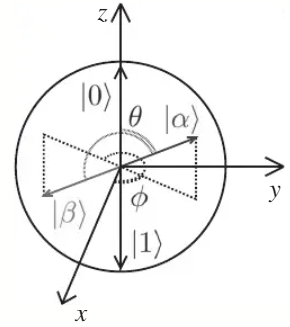
\includegraphics[width=0.3\linewidth]{Immagini - Capitolo 2/Bloch sphere.png}
        \caption{Bloch sphere.}
        \label{fig: Bloch sphere}
    \end{figure}
    Parametrising the states in terms that opposite points on the Bloch sphere correspond to orthogonal states. In general, given a generic qubit state $\ket{\alpha}$, described by parameters $\theta$ and $\phi$, the antipodal point of the corresponding Bloch vector corresponds to angles $(\pi - \theta)$ and $(\phi + \pi)$, respectively, and is associated with the qubit 
    \begin{equation}
        \begin{split}
            \ket{\beta} &= \cos{\bigg(\frac{\pi - \theta}{2}\bigg)}\ket{0} + e^{i(\phi + \pi)}\cos{\bigg(\frac{\pi - \theta}{2}\bigg)}\ket{1} \\
            &= \sin{\bigg(\frac{\theta}{2}\bigg)}\ket{0} - e^{i\phi}\cos{\bigg(\frac{\theta}{2}\bigg)}\ket{1},
        \end{split}
    \end{equation}
    and it is then straightforward to show that 
    \begin{equation}
        \begin{split}
            \mybraket{\beta}{\alpha} &= \bigg[\sin{\bigg(\frac{\theta}{2}\bigg)}\bra{0} - e^{-i\phi}\cos{\bigg(\frac{\theta}{2}\bigg)}\bra{1}\bigg]\bigg[\cos{\bigg(\frac{\theta}{2}\bigg)}\ket{0} + e^{i\phi}\sin{\bigg(\frac{\theta}{2}\bigg)}\ket{1}\bigg] \\
            &= 0.
        \end{split}
    \end{equation}
    Thus, moving from one orthonormal basis to another orthonormal one corresponds to a rotation on the Bloch sphere.
\end{ex}
The expression 
\begin{equation}
    f(\vv) = \sum_{i,j = 1}^n f_i\ve_i^*(v_j\ve_j) = \sum_{i,j = 1}^n f_iv_j\ve_i^*(\ve_j) = \sum_{i=1}^n f_iv_i
\end{equation}
can be interpreted as an inner product defined as
\begin{equation}
\label{eq: inner product}
    \inner{\cdot}{\cdot} : V^* \times V \to \C,\quad (f,\vv) \mapsto \inner{f}{\vv} = f(\vv) = \sum_{i=1}^n f_iv_i.
\end{equation}
It is important to note that the inner product defined in equation \eqref{eq: inner product} is formally different from the scalar product $\mybraket{\cdot}{\cdot} : V \times V \to \C$. Whereas the scalar product receives as its arguments an ordered pair of vectors $(\vv,\vw)$, the arguments of the inner product are a dual vector $f$ and vector $\vv$. 

Consider now two vector spaces $V$ and $W$, and the linear map $f : V \to W$; furthermore, let $g$ be a linear function $g : W \to \C$, namely $g \in W^*$. Then, also the composition map $g \circ f : V \to \C$ is linear, namely $g \circ f \in V^*$. This can be rephrased by saying that the linear map $f : V \to W$ induces a map $f^*$ from the dual vector spaces of $W$ and $V$ that is defined as
\begin{equation}
    f^* : W^* \to V^*,\quad g \mapsto g \circ f,
\end{equation}
where $f^*$ is called the pull-back of $g$. Note that for every $\vv \in V$, one can use the inner product defined in equation \eqref{eq: inner product} to define a linear function such as
\begin{equation}
    \omega_{\vv} : V^* \to \C,\quad f \mapsto \omega_{\vv}(f) = \inner{f}{\vv}.
\end{equation}
The bilinearity of the inner product implies that $\omega_{\vv}$ is an element of $V^{**}$, the dual of the dual of the vector space $V$. In fact, it is instructive to prove that every element of $V^{**}$, namely every linear function from $V^*$ to $\C$ can be constructed in this way, meaning associated with a vector $\vv \in V$. Thus, $V^{**}$ can be identified with the vector space $V$ itself, so $V^{**} \equiv V$. One can then define an action of a vector $\vv$ on a dual vector $f$ by
\begin{equation}
    \vv : V \to \C,\quad f \mapsto \vv(f) = \inner{f}{\vv} = f(\vv).
\end{equation}
Given a complex vector space $V$, one can generalise the notion of vector and dual vector and introduce a tensor of type $(p,q)$, also called a $(p,q)$-tensor defined as the following. 
\begin{defn}[$(p,q)$-tensor]
    Given a complex vector space $V$, a tensor $T$ of type $(p,q)$ is defined as a function of $p$ dual vectors and $q$ vectors that is multilinear, namely that is linear in each of its arguments, such that 
    \begin{equation}
        T : V^* \times \underbrace{\cdots}_{p\,\mathrm{times}} \times V^* \times V \times \underbrace{\cdots}_{q\,\mathrm{times}} \times V \to \C.
    \end{equation}
\end{defn}
Every linear combination $aT + bU$ of $(p,q)$-tensors $T$ and $U$ is also a $(p,q)$-tensor, hence tensors of type $(p,q)$ form a vector space; this follows from the fact that linear combinations preserve the multilinearity of the $(p,q)$-tensor. In general, the components of a $(p,q)$-tensor are defined as
\begin{equation}
    T^{i_1\cdots i_p}_{j_1\cdots j_q} = T(\ve_{i_1}^*,\dots,\ve_{i_p}^*,\ve_{j_1},\dots,\ve_{j_q}),
\end{equation}
and have $p$ upper indices and $q$ lower indices. Note also that the components of a tensor form a multidimensional array, generalising the two-dimensional array of a matrix. Tensors with more indices can be constructed from tensors with fewer indices through the tensor product operation defined as the following.
\begin{defn}[tensor product]
    Let $R$ be a tensor of type $(p,q)$ and let $S$ be a tensor of type $(l,m)$. Their tensor product $T = R \ot S$ is defined as the tensor of type $(p + l, q + m)$ such that 
    \begin{multline}
    \label{eq: tensor product of tensors}
        T(f_1,\dots,f_p,f_{p + 1},\dots,f_{p + l},\vv_1,\dots,\vv_q,\vv_{q + 1},\dots,\vv_{q+m}) = \\
        =R(f_1,\dots,f_p,\vv_1,\dots,\vv_q)S(f_{p + 1},\dots,f_{p + l},\vv_{q + 1},\dots,\vv_{q+m}).
    \end{multline}
\end{defn}
Note that the tensor product is a bilinear operation 
\begin{multline}
    (a_1R_1 + a_2R_2) \ot (b_1S_1 + b_2S_2) = \\
    = a_1b_1(R_1 \ot S_1) + a_1b_2(R_1 \ot S_2) + a_2b_1(R_2 \ot S_1) + a_2b_2(R_2 \ot S_2),
\end{multline}
for all coefficients $a_1,a_2,b_1,b_2 \in \C$. In terms of components the tensor product can be written as
\begin{equation}
\label{eq: tensor product of tensors in terms of components}
    T^{i_1\cdots i_pi_{p + 1}\cdots i_{p + l}}_{j_1\cdots j_qj_{q+1}\cdots j_{q+m}} = R^{i_1\cdots i_p}_{j_1\cdots j_q}S^{i_{p + 1}\cdots i_{p + l}}_{j_{q + 1}\cdots j_{q + m}}.
\end{equation}
One can perform repeated tensor products; the tensor product is associative 
\begin{equation}
    R \ot S \ot T = (R \ot S) \ot T = R \ot (S \ot T).
\end{equation}
Finally, one can define the operation of contraction of a tensor. This is an operation that, when applied to a $(p,q)$-tensor $T$ produces a tensor of type $(p - 1,q - 1)$denoted as $T_{c(ij)}$ and defined as
\begin{multline}
    T_{c(ij)}(f_1,\dots,f_{p - 1},\vv_1,\dots,\vv_{q - 1}) = \\ 
    = \nsum_{k}T(f_1,\dots,\underbrace{\ve_k^*}_{i\mathrm{th}},\dots,f_{p - 1},\vv_1,\dots,\underbrace{\ve_k}_{j\mathrm{th}},\dots,\vv_{q - 1}).
\end{multline}
Note that the sum over $k$ on the right-hand side of the previous expression can be rewritten in component form as 
\begin{equation}
    T_{c(ij)\,m_1\cdots m_{q - 1}}^{l_1\cdots l_{p - 1}} = \nsum_k T^{l_1\cdots l_{i - 1}l_kl_i\cdots l_{p - 1}}_{m_1\cdots m_{j - 1}m_km_j\cdots m_{q - 1}}.
\end{equation}
Thus, in contraction one chooses the $i$th upper index and the $j$th lower index to be the same label $k$, which is then summed over. 

\subsection{Tensor product of vector spaces}
As stated above, $(p,q)$-tensors form a vector space. One can arrive at this conclusion from another point of view.
\begin{defn}[tensor product of vector spaces]
    Let $V$ and $W$ be vector spaces, with $\dim{V} = n$ and $\dim{W} = m$, denoted as $V \ot W$, is the set of all finite linear combinations of tensor products $\vv \ot \vw$ with $\vv \in V$ and $\vw \in W$. If $\{\ve_i\}$ is a basis of $V$ and $\{\vf_j\}$ is a basis of $W$, then 
    \begin{equation}
        V \ot W = \sum_{i=1}^n\sum_{j=1}^m\lambda^{ij}(\ve_i \ot \vf_j),\quad \lambda^{ij} \in \C.
    \end{equation}
\end{defn}
From the tensor product definition one can see that
\begin{equation}
    \dim{(V \ot W)} = nm.
\end{equation}
An element of $V \ot W$ that can be written as $\vv \ot \vw$ for some $\vv \in V$ and $\vw \in W$ is called a ``pure tensor'' or a ``simple tensor''. Note that not all elements of $V \ot W$ are simple.
\begin{ex}
    The state 
    \begin{equation}
        \ket{\psi} = \frac{1}{\sqrt{2}}\ket{0}\ket{0} + \frac{1}{\sqrt{2}}\ket{1}\ket{1}
    \end{equation}
    is not a pure tensor, since it cannot be written as a tensor product 
    \begin{equation}
        (a\ket{0} + b\ket{1})(c\ket{0} + d\ket{1})
    \end{equation}
    for any choice of complex coefficients $a$, $b$, $c$ and $d$. Indeed this tensor product can be rewritten as
    \begin{equation}
        ac\ket{0}\ket{0} + ad\ket{0}\ket{1} + bc\ket{1}\ket{0} + bd\ket{1}\ket{1}
    \end{equation}
    and, if this expression were equal to the state $\ket{\psi}$, then the following conditions should hold
    \begin{equation}
        \begin{cases}
            ac = bd = \dfrac{1}{\sqrt{2}} \\[1.5ex]
            ad = bc = 0 \\
        \end{cases}.
    \end{equation}
    It is easy to see that there exists no solution to this system of equations: the first equation implies that neither $a$ nor $c$ can be zero; since $a$ is different from zero, $ad = 0$ implies that $d = 0$, but then $bd = 1/\sqrt{2}$ does not have any solution. 
\end{ex}
Note that, in general, $V \ot W \neq W \ot V$. However, they are isomorphism vector spaces. This follows from both having the same dimension, or by constructing an explicit isomorphic. In a similar fashion, one can construct the tensor products of dual vector spaces $V^* \ot W^*$ and of a vector space and a dual vector space $V \ot W^*$. This is easiest using a basis and a dual basis
\begin{align}
    V^* \ot W^* &= \sum_{i=1}^n\sum_{j=1}^m\lambda_{ij}(\ve^{*i} \ot \vf^{*j}),\quad \lambda_{ij} \in \C, \\
    V \ot W^* &= \sum_{i=1}^n\sum_{j=1}^m\lambda_j^i(\ve_i \ot \vf^{*j}),\quad \lambda_i^j \in \C.
\end{align}
Note that elements $L = \sum_{i=1}^n\sum_{j=1}^m\lambda_j^i(\ve_i \ot \vf^{*j})$ of $V \ot W^*$ are linear operators $L : W \to V$. This can be seen by denoting 
\begin{equation}
    L = \sum_{i=1}^n\sum_{j=1}^m\lambda_j^i\ket{i}\bra{j}
\end{equation}
and by expanding a vector $\ket{\chi} \in W$ in the basis $\ket{j}$ such that $\ket{\chi} = \sum_{k=1}^m\chi_k\ket{k}$, then $L$ acts on it by 
\begin{equation}
    L\ket{\chi} = \sum_{i=1}^n\sum_{j=1}^m\sum_{k=1}^n\lambda^i_j\chi_k\ket{i}\mybraket{j}{k} = \sum_{i=1}^n\sum_{j=1}^m\lambda^i_j\chi_j\ket{i},
\end{equation}
so $L\ket{\chi}$ is a vector in $V$ with components $\sum_{j=1}^m\lambda^i_j\chi_j$, indexed by the free index $i$. Since the tensor product space is a vector space, one can perform a tensor product of that with another vector space. The tensor product is associative, in the sense that is a natural isomorphism $(V_1 \ot V_2) \ot V_3 \simeq V_1 \ot (V_2 \ot V_3)$, so that one can write $V_1 \ot V_2 \ot V_3$ for short. Now, $(p,q)$-tensors can be defined in an alternative way by first defining a vector space
\begin{equation}
    T^p_q(V) = V \ot \underbrace{\cdots}_{p\,\mathrm{times}} \ot V \ot V^* \ot \underbrace{\cdots}_{q\,\mathrm{times}} \ot V^*.
\end{equation}
Using the basis, elements $T \in T^p_q(V)$ can be expanded as
\begin{equation}
    T = \sum_{\substack{i_1,\dots,i_p \\ j_1,\dots,j_q}}T^{i_1\cdots i_p}_{j_1\cdots j_q}(\ve_{j_1} \ot \cdots \ot \ve_{i_p} \ot \ve_{*j_1} \ot \cdots \ot \ve_{*j_q}).
\end{equation}
Hence, the elements $T \in T^p_q(V)$ can be recognised as $(p,q)$-tensors; this can be taken as their alternative definition. Acting with $T$ on the basis vectors projects out its components $T^{i_1\cdots i_p}_{j_1\cdots j_q}$. 
\begin{notz}
    At this point the Einstein summation convention will be used: repeated indices are understood to be summed over, and the explicit summation symbols $\Sigma$ are not shown. Thus, for example one has
    \begin{equation}
        T = T^{i_1\cdots i_p}_{j_1\cdots j_q}(\ve_{j_1} \ot \cdots \ot \ve_{i_p} \ot \ve^{*j_1} \ot \cdots \ot \ve^{*j_q}).
    \end{equation}
\end{notz}
The tensor components satisfy a characteristic transformation rule under a change of basis. For notational brevity, consider only a $(1,2)$-tensor. Let $\ve_k' = R_k^l\ve_l$ and $\vf^{*i} = S^i_j\ve^{*j}$ be the transformation between two orthonormal bases $\{\ve_i\}$ and $\{\ve_i'\}$. Since $\vf^{*i}(\vf_k) = \ve^{*i}(\ve_k) = \delta^i_k$, one must have
\begin{equation}
    \delta^i_k = \vf^{*i}(\ve_k') = S^i_jR^l_ke^{*j}(\ve_l) = S^i_jR^l_K\delta^j_l = S^i_jR^j_k,
\end{equation}
which means that $S$ is the inverse of $R$, namely $S^i_j = (R^{-1})^i_j$. Denoting the components of a $(1,2)$-tensor in the two bases as $T^i_{jk}$ and $T'^{i}_{jk}$, one gets
\begin{equation}
    \begin{split}
        T &= T'^i_{jk}(\vf_i \ot \vf^{*j} \ot \vf^{*k}) \\
        &= T'^i_{jk}R^l_i(R^{-1})^j_m(R^{-1})^k_n(\ve_l \ot \ve^{*m} \ot \ve^{*n}) \\
        &= T^l_{mn}(\ve_l \ot \ve^{*m} \ot \ve^{*n}),
    \end{split}
\end{equation}
so that the components transform as
\begin{equation}
    T^l_{mn} = R^l_i(R^{-1})^j_m(R^{-1})^k_nT'^i_{jk}.
\end{equation}
Transformation rules for other $(p,q)$-tensors can be derived in a similar manner. 
\begin{notz}
    It is convenient to introduce a tensor power notation; given a non-negative integer $n$, one can write
    \begin{equation}
        V^{\ot n} = V \ot \underbrace{\cdots}_{n\,\mathrm{times}} \ot V,
    \end{equation}
    which can be used to write $T^p_q(V) = V^{\ot p} \ot V^{*\ot q}$.
\end{notz}
Let's now consider the tensor product defined in equation \eqref{eq: tensor product of tensors}. It should correspond to the product map $T^p_q(V) \ot T^m_n(V) \to T^{p + m}_{q + n}(v)$. There is one subtlety in making contact with equation \eqref{eq: tensor product of tensors}. Consider, for example, the tensor product of a $(1,1)$-tensor $R$ with a $(1,0)$-tensor $S$. At first one can attempt 
\begin{equation}
    R \ot S = (R^i_j\ve_i \ot \ve^{*j}) \ot (S^k\ve_k) = R^i_jS^k\ve_i \ot \ve^{*j} \ot \ve_k.
\end{equation}
However, the expansion of a $(2,1)$-tensor involves the basis vectors $\ve_i \ot \ve_j \ot \ve^{*k}$ rather than $\ve_i \ot \ve^{*j} \ot \ve_k$, and the tensor product is not commutative. One has to define the tensor product $R \ot S$ in such a way that all basis vectors of $V$ and dual basis vectors of $V^*$ are grouped together. That is, instead what first attempted one defines
\begin{equation}
    R \ot S = R^i_kS^j(\ve_i \ot \ve_j \ot \ve^{*k}).
\end{equation}
Now, consider again a $(p,q)$-tensor $R$ and a $(m,n)$-tensor $S$. Expanding both
\begin{align}
    R &= R^{i_1\cdots i_p}_{j_1\cdots j_q}(\ve_{i_1} \ot \cdots \ot \ve_{i_p} \ot \ve^{*j_1} \ot \cdots \ot \ve^{*j_q}), \\
    S &= S^{k_1\cdots k_p}_{l_1\cdots l_q}(\ve_{k_1} \ot \cdots \ot \ve_{k_p} \ot \ve^{*l_1} \ot \cdots \ot \ve^{*l_q}),
\end{align}
the tensor product $T = R \ot S$ can be built as
\begin{equation}
    \begin{split}
        T &= R^{i_1\cdots i_p}_{j_1\cdots j_q}S^{k_1\cdots k_m}_{l_1\cdots l_n}(\ve_{i_1} \ot \cdots \ot \ve_{i_p} \ot \ve_{k_1} \ot \cdots \ot \ve_{k_m} \\
        &\ot \ve^{*j_1} \ot \cdots \ot \ve^{*j_q} \ot \ve^{*l_1} \ot \cdots \ve^{*l_n}) \\
        &= R^{i_1\cdots i_p}_{j_1\cdots j_q}S^{i_{p + 1}\cdots i_{p + m}}_{j_{q + 1}\cdots j_{q + n}}(\ve_{i_1} \ot \cdots \ot \ve_{i_p} \ot \ve_{i_{p + 1}} \ot \cdots \ot \ve_{i_{p + m}} \\
        &\ot \ve^{*j_1} \ot \cdots \ot \ve^{*j_q} \ot \ve^{*j_{q + 1}} \ot \cdots \ve^{*j_{q + m}}),
    \end{split}
\end{equation}
in agreement with equation \eqref{eq: tensor product of tensors in terms of components}.

\subsection{Tensor product of linear operators}
Since elements $L \in W \ot V^*$ are linear operators $L : V \to W$, conversely one can represent every linear operator from $V$ to $W$ in a tensor product basis. Let $\{\ve_i\}$ be an orthonormal basis in $V$ and let $\{\vf_k\}$ be an orthonormal basis of $W$. Every linear operator $A : V \to W$ is then uniquely determined by its components with respect to the two bases. One can then identify the linear operator with the matrix having these components as its entries, $A = (A)^i_j$. One way to explicitly extract the components is to use the scalar product in $W$ and let $A$ act on the basis vector of $V$ by
\begin{equation}
    A^i_j = \mybraket{\vf_i}{A\ve_j}.
\end{equation}
Another way to extract the components of $A$ is to use the dual basis $\{\vf^{*i}\}$ of $W^*$ and compute the inner products
\begin{equation}
    A^i_j = \mybraket{\vf^{*i}}{A\ve_j}.
\end{equation}
When acting on a vector $\vv = v^k\ve_k \in V$, it gives
\begin{equation}
    A\vv = A^i_J\vf_i\ve^{*j}(v^k\ve_k) = A^i_jv^k\vf_i\ve^{*j}(\ve_k) = A^i_jv^k\delta^j_k\vf_i = A^i_j\ve^j\vf_i,
\end{equation}
which is a vector of $W$ with components $A^i_jv^j$, as expected. Note the product of the matrix $(A)^i_j$ and the vector $\vv^j$. In quantum mechanics it is often very useful to construct tensor products of linear operators. 
\begin{defn}[tensor product of linear operators]
    Let $A : V_1 \to V_2$ and $W : W_1 \to W_2$ be two linear operators. The tensor product of linear operators is defined by first imposing the action on the simple tensor of $V_1 \ot W_1$ as
    \begin{equation}
        (A \ot B)(\vv \ot \vw) = A(\vv) \ot B(\vw),\quad \forall \vv \ot \vw \in V_1 \ot W_1;
    \end{equation}
    next, choosing a basis $\basis_{V_1} = \{\ve_i\}$ and $\basis_{W_1} = \{\vf_j\}$, by imposing the action of $(A \ot B)$ on a generic $(2,0)$-tensor $T = T^{ij}(\ve_i \ot \vf_j)$ in $V_1 \ot W_1$ as
    \begin{equation}
        A \ot B : V_1 \ot W_1 \to V_2 \ot W_2,\quad T \mapsto (A \ot B)(T) = T^{ij}A(\ve_i) \ot B(\vf_j);
    \end{equation}
    thus, expanding the linear operators in a basis, the expansion of their tensor product becomes
    \begin{equation}
        A \ot B = A^i_jB^k_l(\ve_i \ot \ve_k \ot \vf^{*j} \ot \vf^{*l})
    \end{equation}
\end{defn}
As before, the next step is to generalise this definition to multiple tensor products of linear operators. Let $T \in V_1 \ot \cdots \ot V_n$, then 
\begin{equation}
    (A_1 \ot \cdots \ot A_n)(T) = T^{i_1\cdots i_n}A_1(\ve_{i_1}) \ot \cdots \ot A_n(\ve_{i_n}),
\end{equation}
where $A_k$ are linear operators $A_k : V_k \to W_k$. Generalising further, one can then form linear combinations of tensor products of linear operators, to construct more general linear operators acting on $V_1 \ot \cdots \ot V_n$. Let $\{A_k^{(r)}\}$, with $r = 1,\dots,s$, be a collection of linear operators from $V_k$ to $W_k$, then the operator $A$ is defined a 
\begin{equation}
    A = \sum_{r=1}^sc_r(A_1^{(r)} \ot \cdots \ot A_n^{(r)}),\quad c_r \in \C,
\end{equation}
is a linear operator $A : V_1 \ot \cdots \ot V_n \to W_1 \ot \cdots \ot W_n$. For this type of generic operator $A$ acting on a tensor product of vectors spaces, there is no reason to try to break up its components into a sum of products; instead, one can use the generic tensor component notation and write
\begin{equation}
    A = A^{i_1\cdots i_n}_{j_1\cdots j_n}\ket{i_1,\dots,i_n}\bra{j_1,\dots,j_n}.
\end{equation}
The tensor product is closely related to the Kronecker product of matrices, defined as the following.
\begin{defn}[Kronecker product]
    Let $A$ be an $N \times N$ matrix with components $a_{ij}$ and let $B$ be an $M \times M$ matrix with components $b_{ij}$. The Kronecker product $A \ot B$ of the matrices is defined to be an $NM \times NM$ matrix with the structure
    \begin{equation}
        \begin{split}
            A \ot B &= 
            \begin{pmatrix}
                a_{11} & \cdots & a_{1N} \\
                \vdots & \ddots & \vdots \\
                a_{N1} & \cdots & a_{NN}
            \end{pmatrix} \ot
            \begin{pmatrix}
                b_{11} & \cdots & b_{1M} \\
                \vdots & \ddots & \vdots \\
                b_{M1} & \cdots & b_{MM}
            \end{pmatrix} \\
            &= 
            \begin{pmatrix}
                a_{11}B & \cdots & a_{1N}B \\
                \vdots & \ddots & \vdots \\
                a_{N1}B & \cdots & a_{NN}B
            \end{pmatrix} \\
            &= 
            \begin{pmatrix}
                a_{11}b_{11} & \cdots & a_{11}b_{1M} & a_{12}b_{11} & \cdots & a_{1N}b_{1M} \\
                \vdots & \ddots & \vdots & \vdots & \ddots & \vdots \\
                a_{N1}b_{M1} & \cdots & a_{N1}b_{MM} & a_{N2}b_{M1} & \cdots & a_{NN}b_{MM}
            \end{pmatrix}.
        \end{split}
    \end{equation}
\end{defn}
The Kronecker product of two matrices in not commutative, namely $A \ot B \neq B \ot A$, but the two resulting matrices can be mapped into each other by a permutation of rows and columns. Furthermore, the Kronecker $\vv \ot f$ between a vector and a dual vector yields an $N \times N$ matrix
\begin{equation}
    \vv \to f =
    \begin{pmatrix}
        v^1 \\
        \vdots \\
        v^N
    \end{pmatrix} \ot
    \begin{pmatrix}
        f_1,\dots,f_N
    \end{pmatrix} = 
    \begin{pmatrix}
        v^1f_1 & \cdots & v^1 \\
        \vdots & \ddots & \vdots \\
        v^Nf_1 & \cdots & v^Nf_N
    \end{pmatrix}.
\end{equation}
In a similar way, the Kronecker product of a vector $\vv$ with $N$ components and a vector $\vw$ with $M$ components is a vector with $NM$ components
\begin{equation}
    \vv \ot \vw = 
    \begin{pmatrix}
        v^1 \\
        \vdots \\
        v^N
    \end{pmatrix} \ot 
    \begin{pmatrix}
        w^1 \\
        \vdots \\
        w^M
    \end{pmatrix} =
    \begin{pmatrix}
        v^1\vw \\
        \vdots \\
        v^N\vw
    \end{pmatrix} = 
    \begin{pmatrix}
        v^1w^1 \\
        \vdots \\
        v^1w^M \\
        \vdots \\
        v^Nw^1 \\
        \vdots \\
        v^Nw^M
    \end{pmatrix}.
\end{equation}
Likewise, a product of a dual row vector $f$ with $N$ components and a dual row vector $g$ with $M$ components is a dual row vector with $NM$ components. Now, let $A$ be a linear operator on $V$ with $\dim{V} = N$ and $B$ a linear operation on $W$ with $\dim{W} = M$. Given a basis in $V$ and one in $W$, the operators can be identified with the matrices of their coefficients and their tensor product $A \ot B$ becomes the Kronecker product of the matrices, resulting in an $NM\times NM$ matrix. The trace of this matrix is taken over the tensor product basis $\{\ket{i},\ket{j}\}$, with $1 \le i \le N$ and $1 \le j \le M$, of $V \ot W$ as
\begin{equation}
    \begin{split}
        \tr{(A \ot B)} = \sum_{i=1}^N\sum_{j=1}^M\mybrakett{i}{\mybrakett{i}{(A \ot B)}{j}}{j} &= \sum_{i=1}^N\sum_{j=1}^M\mybrakett{i}{A}{i}\mybrakett{j}{B}{j} \\
        &= \sum_{i=1^N}\mybrakett{i}{A}{i}\sum_{j=1}^M\mybrakett{j}{B}{j},
    \end{split}
\end{equation}
from where it is immediate to see the property of the trace
\begin{equation}
    \tr{(A \ot B)} = \tr{(A)}\tr{(B)}.
\end{equation}
A similar property holds for the determinant of said matrix, in particular
\begin{equation}
    \det{(A \ot B)} = (\det{A})^M(\det{B})^N.
\end{equation}

\subsection{Heisenberg spin chain}
The quantum Heisenberg spin chain is an elementary model of magnets. A ferromagnetic material can be thought of as consisting particles with a magnetic moment. When the alignment of the elementary magnets has a preferred direction, which is observable on a macroscopic scale the material appears to be magnetic. At the microscopic level, the existence of the magnetic moments can be interpreted in terms of the spin of particles; for example, an electron acts like a tiny bar magnet with a dipole magnetic field, associated with a magnetic moment $\vmu = -g_s\mu_Bm\vs$, where $g_s$ is called the spin $g$-factor, $\mu_B$ is the Bohr magneton and $m = \pm1/2$ is the spin quantum number. Quantum Heisenberg spin chains are models of one-dimensional lattices of elementary magnetic moments, with nearest-neighbour interactions that tend to make neighbouring magnetic moments aligned an parallel, or aligned and oppositely oriented, resulting in a net magnetisation. Start by considering linear operation of the form 
\begin{equation}
\label{eq: linear operator (Heisenberg spin chain)}
    \MI_2 \ot \cdots \ot \MI_2 \ot \sigma^a_k \ot \sigma^b_{k + 1} \ot \MI_2 \cdots \ot \MI_2,
\end{equation}
where the subscripts $k$ and $k + 1$ have been to the Pauli matrices to emphasize that they act on the electrons at the $k$th site and the $(k + 1)$th site, respectively. Acting on a basis state
\begin{equation}
    \ket{i_1\cdots i_{k-1}i_ki_{k+1}\cdots i_N} = \ket{i_1} \ot \cdots \ot \ket{i_{k-1}} \ot \ket{i_k} \ot \ket{i_{k+1}} \ot \cdots \ot \ket{i_N}
\end{equation}
the operator defined in equation \eqref{eq: linear operator (Heisenberg spin chain)} produces the state
\begin{equation}
    \ket{i_1} \ot \cdots \ot \ket{i_{k-1}} \ot \sigma^a\ket{i_k} \ot \sigma^b\ket{i_{k+1}} \ot \cdots \ot \ket{i_N}.
\end{equation}
Suppressing the unit matrices in the definition of the operator introduced in equation \eqref{eq: linear operator (Heisenberg spin chain)} for a shorter notation, one can define a set of local operators, labelled by $k$, of the form
\begin{equation}
\label{eq: set of local linear operators (Heisenberg spin chain)}
    \hatH_{k,k + 1} = \frac{\lambda}{2}\bigg(\MI_k \ot \MI_{k + 1} - \sum_{a=1}^3\sigma^a_k \ot \sigma^a_{k + 1}\bigg),
\end{equation}
where $\lambda \in \R$ is a parameter controlling the strength and alignment of the nearest-neighbour interactions. Finally, by summing over the sites, one constructs the Hamiltonian operator as
\begin{equation}
    \hatH = \sum_{k=1}^{N-1}\hatH_{k,k + 1}.
\end{equation}
This is the Heisenberg XXX quantum spin chain. Note that there exist other variants of Heisenberg spin chains, with different Hamiltonian operators. Also, one can either assume the sites to be arranged in a periodic chain, identifying the first and the $N$th site, and letting the sum run up to $N$, which yields a closed spin chain, or having an infinite lattice with the sum running over all integers, which corresponds to an infinite chain. The Hamiltonian has a discrete set of degenerate eigenvalues $E_n$ and eigenstates $\ket{\psi_n}$, which satisfy 
\begin{equation}
    \hatH\ket{\psi_n} = E_n\ket{\psi_n}.
\end{equation}
When $\lambda > 0$, the interaction defined in equation \eqref{eq: set of local linear operators (Heisenberg spin chain)} tends to align the neighbouring spins: in that case, the interaction and the resulting ground state, with energy $E_0$, are said to be ferromagnetic; conversely, for $\lambda < 0$, the interaction and the ground state are called anti-ferromagnetic. The model has a $SU(2)$ symmetry which helps in finding and organising the eigenstates. Defining
\begin{equation}
    J^a = \frac{1}{2}\sum_{k=1}^N\sigma^a_k,
\end{equation}
it is easy to see that $J^a$ operators satisfy the commutation relations of the generators of the $SU(2)$ Lie group $\comm{J^a}{J^b} = i\epsilon^{abc}J^c$. Moreover, one can show that they commute with the Hamiltonian, $\comm{J^a}{H} = 0$ for any $a \in \{1,2,3\}$. This means that the Heisenberg XXX spin chain has an $SU(2)$ symmetry, then the energy eigenstates for every $E_n$ correspond to irreducible spin-$j$ representations of the $SU(2)$ group. Note that the discussion started with the smallest irreducible two-dimensional representation for a single electron, but as a result of taking $N$ copies it ended with a $2^N$-dimensional vector space $V$. The action of $SU(2)$ on $V$ is reducible. Since every state can be expressed in the basis of energy eigenstates, which belong to irreducible representations, studying the energy eigenstates of this system corresponds to solving the reduction problem.
